\chapter{PERSPECTIVAS DE LA DEUDA Y NECESIDAD DE CONSOLIDACION FISCAL}\label{chap:perspectivas}

La crisis sanitaria provocada por la pandemia dejó profundas cicatrices en la economía colombiana, exacerbando desafíos fiscales preexistentes y generando nuevas presiones sobre las finanzas públicas. El aumento del gasto primario en el PIB que se produjo durante la pandemia aún no se ha revertido y no ha estado acompañado por un incremento proporcional en los ingresos fiscales. Como resultado, el país enfrenta un déficit persistente y un creciente nivel de deuda, lo que, a su vez, ha elevado el pago de intereses y agravado el desbalance fiscal. Ante un panorama marcado por un alto endeudamiento y déficits persistentes, resulta imperativo implementar un plan de consolidación fiscal que reduzca el déficit y estabilice la deuda. Esto requiere una estrategia que combine un aumento en los ingresos tributarios con un recorte del gasto, como se argumenta en este capítulo. 

\section{Proyecciones de deuda y balance}

Los resultados fiscales de 2024, independientemente de su alineación con la regla fiscal, confirman una tendencia: la deuda se acerca cada vez más a niveles insostenibles. No obstante, aún se está a tiempo para implementar un ajuste fiscal que reviertan esta tendencia, como se infiere de los posibles escenarios para la evolución de la deuda pública que se presentan a continuación.

\begin{figure}[h!]
\centering
\caption{Proyecciones de Deuda Neta del GNC}\label{fig:consolida}

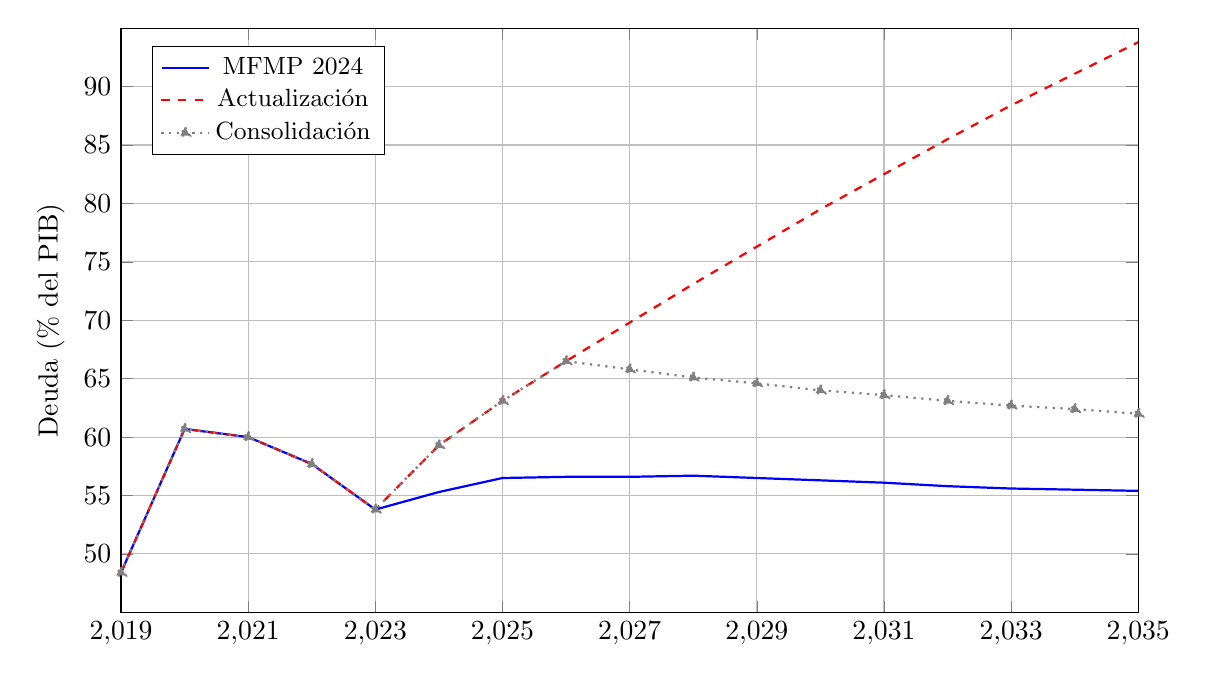
\begin{tikzpicture}
    \begin{axis}[
        width=14.5cm, height=9cm,
%        xlabel={A\~{n}o},
        ylabel={Deuda (\% del PIB)},
        xmin=2019, xmax=2035,
        ymin=45, ymax=95,
        xtick={2019,2021,...,2035},
%        xticklabel style={rotate=90,anchor=east},
        ytick={50,55,...,90},
        legend pos=north west,
        grid=major,
        legend style={font=\small}
    ]

    % Deuda MFMP 2024
    \addplot[
        color=blue, thick
    ] coordinates {
        (2019,48.4) (2020,60.7) (2021,60.0) (2022,57.7) (2023,53.8) 
        (2024,55.3) (2025,56.5) (2026,56.6) (2027,56.6) (2028,56.7) 
        (2029,56.5) (2030,56.3) (2031,56.1) (2032,55.8) (2033,55.6) 
        (2034,55.5) (2035,55.4)
    };
    \addlegendentry{MFMP 2024}

    % Deuda Actualizada
    \addplot[
        color=red, thick, dashed
    ] coordinates {
        (2019,48.4) (2020,60.7) (2021,60.0) (2022,57.7) (2023,53.8) 
        (2024,59.3) (2025,63.1) (2026,66.5) (2027,69.8) (2028,73.1) 
        (2029,76.3) (2030,79.5) (2031,82.5) (2032,85.5) (2033,88.4) 
        (2034,91.1) (2035,93.8) 
    };
    \addlegendentry{Actualizaci\'on}

    % Deuda Consolidación
    \addplot[mark=triangle*, color=gray, thick, dotted ] coordinates {
        (2019,48.4) (2020,60.7) (2021,60.0) (2022,57.7) (2023,53.8) 
        (2024,59.3) (2025,63.1) (2026,66.5) (2027,65.8) (2028,65.1) 
        (2029,64.6) (2030,64.0) (2031,63.6) (2032,63.1) (2033,62.7) 
        (2034,62.4) (2035,62.0) 
    };
    \addlegendentry{Consolidaci\'on}

    \end{axis}
\end{tikzpicture}
%\vspace{0.1cm}
\par\footnotesize{\textit{Fuente: Elaboración propia con base en MFMP 2024, Balance General del GNC y Deuda del GNC, Ministerio de Hacienda.}}
\end{figure}

\begin{figure}[h!]
\centering
\caption{Proyecciones del Balance Primario del GNC}
\label{fig:bp}
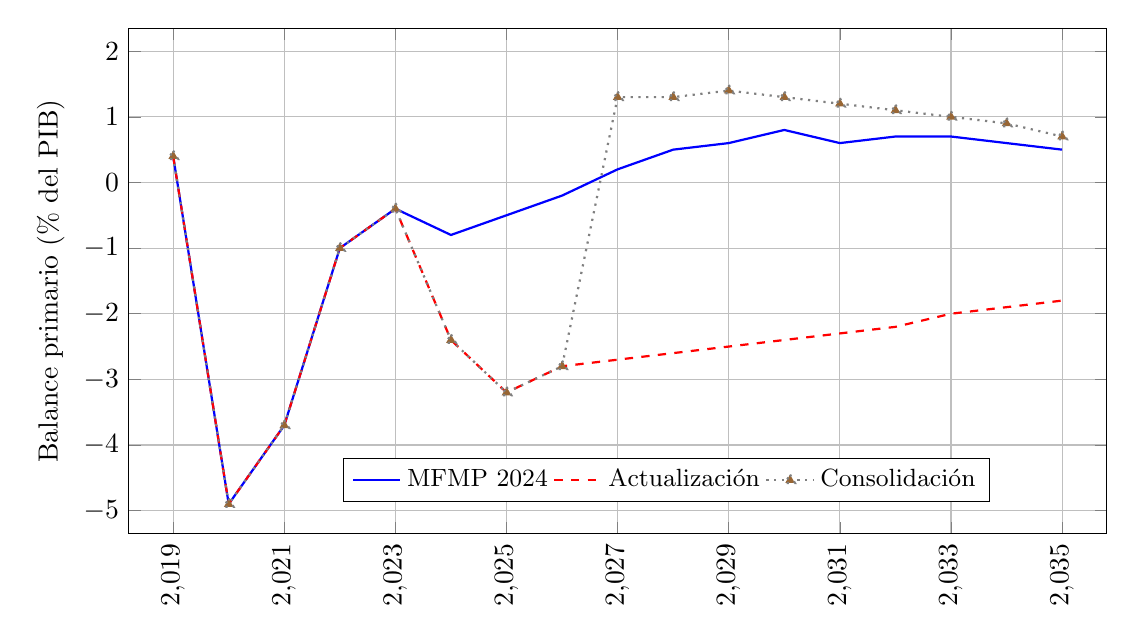
\begin{tikzpicture}
\begin{axis}[
    width=14cm,
    height=8cm,
%    xlabel={Año},
    ylabel={Balance primario (\% del PIB)},
    xmin=2019, xmax=2035,
    ymin=-5, ymax=2,
%    xtick={2019,2020,...,2035},
    xtick={2019,2021,...,2035},
    xticklabel style={rotate=90,anchor=east},
    ytick={-5,-4,-3,-2,-1,0,1,2},
    grid=both,
    legend style={at={(0.55,0.15)},
    legend style={font=\small},
    anchor=north, legend columns=3},
    enlargelimits=0.05,
%    title={Escenarios del balance primario (\% del PIB)}
]

% Datos MFMP
\addplot+[mark=none, color=blue, thick] coordinates {
(2019,0.4) (2020,-4.9) (2021,-3.7) (2022,-1.0) (2023,-0.4)
(2024,-0.8) (2025,-0.5) (2026,-0.2) (2027,0.2) (2028,0.5)
(2029,0.6) (2030,0.8) (2031,0.6) (2032,0.7) (2033,0.7) (2034,0.6) (2035,0.5)
};
\addlegendentry{MFMP 2024}

% Datos Actualización
\addplot+[mark=none, color=red, thick, dashed] coordinates {
(2019,0.4) (2020,-4.9) (2021,-3.7) (2022,-1.0) (2023,-0.4)
(2024,-2.4) (2025,-3.2) (2026,-2.8) (2027,-2.7) (2028,-2.6)
(2029,-2.5) (2030,-2.4) (2031,-2.3) (2032,-2.2) (2033,-2.0) (2034,-1.9) (2035,-1.8)
};
\addlegendentry{Actualización}

% Datos Consolidación
\addplot+[mark=triangle*, color=gray, thick, dotted] coordinates {
(2019,0.4) (2020,-4.9) (2021,-3.7) (2022,-1.0) (2023,-0.4)
(2024,-2.4) (2025,-3.2) (2026,-2.8) (2027,1.3) (2028,1.3)
(2029,1.4) (2030,1.3) (2031,1.2) (2032,1.1) (2033,1.0) (2034,0.9) (2035,0.7)
};
\addlegendentry{Consolidación}
\end{axis}
\end{tikzpicture}
\par\footnotesize{\textit{Fuente: Elaboración propia con base en MFMP 2024, Balance del GNC y Deuda del GNC, Ministerio de Hacienda.}}
\end{figure}


%Con el fin de cuantificar el ajuste fiscal necesario para revertir la tendencia creciente de la deuda pública, se presentan tres escenarios posibles para la deuda pública (Figura \ref{fig:consolida}) y para el balance primario (Figura \ref{fig:bp}). El primer escenario corresponde al escenario oficial del Marco Fiscal de Mediano Plazo (MFMP) de 2024. El segundo escenario refleja una actualización de las trayectorias de deuda y balance con base en los resultados fiscales al cierre de 2024. El tercero plantea un escenario de consolidación fiscal que supone un ajuste lo suficientemente significativo como para que la deuda retome una senda decreciente y se acerque lo suficiente al ancla del 55\% del PIB en 2037, una década después del inicio del ajuste necesario para la consolidación fiscal.

Con el objetivo de estimar el ajuste fiscal necesario para revertir la trayectoria creciente de la deuda pública, se presentan tres escenarios alternativos para la evolución de la deuda (Figura \ref{fig:consolida}) y del balance primario (Figura \ref{fig:bp}). El primer escenario corresponde a la proyección oficial del Marco Fiscal de Mediano Plazo (\gls{mfmp}) de 2024. El segundo actualiza dichas trayectorias con base en los resultados fiscales observados al cierre de 2024. El tercero supone un ajuste fiscal lo suficientemente grande para cumplir la regla fiscal a partir de 2027.

El escenario del \gls{mfmp} 2024 corresponde al escenario oficial para mediados de 2024. En este escenario la deuda no se despega significativamente de su ancla del 55\% del PIB. Sin embargo, este escenario no incorpora los riesgos materializados en 2024, en particular la caída aún más grande de lo que se esperaba en los ingresos tributarios y un recorte de gasto que finalmente no fue materializado en el monto que el \gls{mfmp} 2024 exigía.

En el escenario actualizado se supone que la situación fiscal se mantiene tan deteriorada como lo estuvo en 2024.  El gasto primario es el 18,9\% del PIB, tal como en 2024. Los ingresos tributarios son el 14,5\% del PIB en 2025 y crecen 0,1 puntos porcentuales cada año gracias a la gestión adicional de la \gls{dian}. Los demás ingresos toman las misma senda del \gls{mfmp} 2024. Se supone una tasa de interés real del 4\% y una tasa de crecimiento para la economía del 3\%, valores muy cercanos a los promedios históricos estimados por \textcite{zapata2022deuda}. 

Por un lado, la actualización es un escenario ácido en la medida en que hace permanente el mal desempeño fiscal del 2024. Por el otro, es benigno en la medida que mantiene constante la participación del gasto primario en el PIB, un supuesto cuestionable dadas las presiones de gasto que se discuten en el Capítulo \ref{chap:menosgasto}. Adicionalmente, supone una tasa de interés que no incorpora el aumento reciente de la percepción del riesgo país y una tasa de crecimiento de la economía que no incorpora riesgos como la desaceleración de la inversión privada o el envejecimiento de la población (\cite{Parra-Polanía2025}). 

En conjunto, el escenario actualizado es relativamente optimista, dados los supuestos favorables sobre gasto, intereses y crecimiento económico. Esto hace que los resultados sean aún más preocupantes, pues incluso bajo estas condiciones benignas la deuda presenta un crecimiento acelerado. Como lo muestra la Figura \ref{fig:consolida}, para el año 2028 la deuda pública superaría el 71\% del PIB en el escenario actualizado, nivel que la regla fiscal identifica como el umbral a partir del cual la deuda se considera insostenible.

Estos resultados enfatizan la necesidad de implementar la consolidación fiscal de manera gradual pero urgente, antes de que el deterioro de los indicadores fiscales limite aún más la capacidad de respuesta del Estado. Persistir en un déficit elevado sin una senda clara de ajuste entraña riesgos macroeconómicos significativos. Una percepción de debilidad fiscal deterioraría aún más la credibilidad del país, elevando el costo del financiamiento tanto para el sector público como para el privado, con efectos negativos sobre la inversión, el empleo y el crecimiento económico. Además, una mayor percepción de riesgo fiscal podría traducirse en una devaluación del peso, lo que a su vez elevaría el costo del servicio de la deuda externa y presionaría al alza la inflación. En un entorno tan incierto, el espacio de maniobra del Gobierno ante choques externos o internos —como una nueva pandemia o una crisis financiera internacional— se vería gravemente limitado. En escenarios más críticos, la falta de financiamiento por parte de inversionistas privados o de la banca multilateral podría generar presiones para recurrir al banco central, afectando su independencia y generando riesgos inflacionarios adicionales. Finalmente, postergar el ajuste obliga a implementarlo de forma súbita cuando las condiciones ya son adversas, amplificando los costos económicos y sociales del proceso de consolidación fiscal.

%En el escenario de consolidación, el balance primario logra corregirse en 4 puntos del PIB para el año 2029. En particular, se asume que, respecto al escenario actualizado, el balance primario mejora en 2 puntos del PIB en 2027 y en otros 2 puntos en 2029. Este ajuste permite que, una década después de iniciado el ajuste, la deuda pública se acerque lo suficiente a su ancla, definida como el 55\% del PIB. Conviene reiterar que esta ancla se sitúa por encima del promedio histórico de la deuda antes de la pandemia, que era del 39\% del PIB. Desafortunadamente, parece poco factible alcanzar superávits primarios lo suficientemente elevados como para retornar a niveles de deuda comparables a los de la prepandemia, al menos en un futuro previsible. 
 
En el escenario de consolidación, se supone que el balance primario se ajusta de tal forma que a partir de 2027 se cumple con la regla fiscal. Por construcción, el cumplimiento de dicha regla asegura que la deuda pública como porcentaje del PIB converja hacia el ancla del 55\%, garantizando así el retorno a una senda sostenible, como lo muestra la Figura \ref{fig:consolida}. No obstante, según se observa en la Figura \ref{fig:bp}, el cumplimiento estricto de la regla fiscal a partir de 2027 implicaría un ajuste del balance primario de más de cuatro puntos del PIB. Un ajuste de tal magnitud es inviable en un solo año, por lo que la única alternativa realista es implementar el ajuste fiscal de manera gradual a lo largo de varios años. Como referencia, la mayoría de los esfuerzos de consolidación fiscal a nivel internacional implican mejoras anuales del balance primario en el rango de 1 a 2 puntos del PIB (\cite{imfconsolidation2023}).

Alcanzar el nivel de ajuste fiscal necesario para revertir la tendencia de la deuda pública es un desafío considerable. En particular, lograr un ajuste de más de cuatro puntos del PIB es una meta altamente ambiciosa, aún si se trata de implementar a lo largo de varios años. Desafortunadamente, lo más probable es que los esfuerzos fiscales necesarios para estabilizar la deuda pública tengan que ser aún mayores, dadas las amenazas que se vislumbran en términos del crecimiento del gasto, como se discute en el Capítulo \ref{chap:menosgasto}.

%La magnitud del ajuste fiscal que necesita el país obliga a considerar tanto un aumento en el recaudo como una reducción del gasto. Por un lado, la experiencia reciente demuestra que las reformas tributarias en Colombia no han logrado incrementos significativos y sostenidos en el recaudo, por lo cual es difícil aspirar a aumentar el recaudo más allá de dos puntos del PIB. Por otro lado, las restricciones legales que pesan sobre el gasto público hacen inviable  recortes de gasto superiores a dos puntos del PIB, como se argumenta en el Capítulo \ref{chap:menosgasto}. 

%\input{Tablas/Cap04/tax:summ }

%Confiar en que el ajuste fiscal puede basarse exclusivamente en el aumento del recaudo es problemático, dadas las limitaciones históricas de las reformas tributarias en Colombia. En particular, ninguna de las últimas reformas ha aspirado —ni siquiera en su versión inicial presentada al Congreso— a recaudar más de dos puntos del PIB, como se muestra en la Tabla \ref{tab:tax:summ}. En segundo lugar, los resultados efectivos han sido aún más modestos. Como muestra la Figura \ref{fig:Ingreso}, entre 2019 y 2024 el recaudo tributario aumentó apenas 0,4 puntos del PIB, pasando del 14,0 al 14,4\%, a pesar de la aprobación de dos reformas en ese período. Esta experiencia sugiere que las reformas tributarias han tenido un impacto limitado sobre los ingresos fiscales, lo que hace poco realista pensar que un ajuste superior a cuatro puntos del PIB pueda lograrse únicamente por la vía del recaudo.

\section{¿Ajuste de ingresos o ajuste de gastos?}

Confiar en que el ajuste fiscal puede basarse exclusivamente en el aumento del recaudo es problemático, dadas las limitaciones históricas de las reformas tributarias en Colombia. Ninguna de las reformas recientes ha aspirado —ni siquiera en su versión inicial presentada al Congreso— a recaudar más de dos puntos del PIB. Peor aún, los resultados efectivos han sido más modestos. Como muestra la Figura \ref{fig:Ingreso}, entre 2019 y 2024 el recaudo tributario aumentó menos de medio punto del PIB, pasando del 14,0 al 14,4\%, a pesar de la aprobación de dos reformas en ese período. Esta experiencia sugiere que las reformas tributarias han tenido un impacto limitado sobre los ingresos fiscales, lo que hace poco realista pensar que un ajuste superior a cuatro puntos del PIB pueda lograrse únicamente por la vía del recaudo.


%\begin{figure}[h!]
    \centering
    \caption{Inflexibilidades y flexibilidades del Gasto Total del GNC (\% PIB)}
    \label{fig:flexnoflex}
    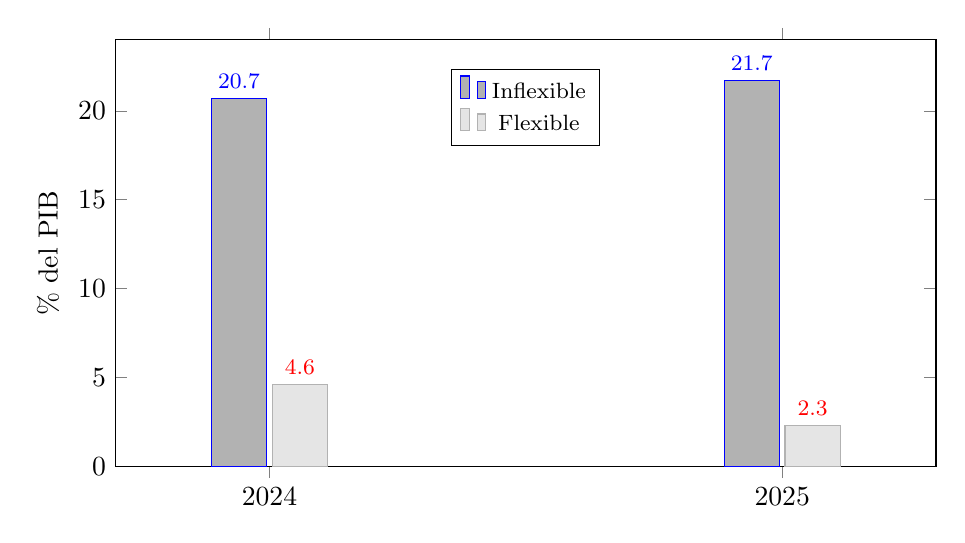
\begin{tikzpicture}
        \begin{axis}[
            ybar,
            bar width=20pt,
            enlarge x limits=0.3,
            ymin=0,
            ymax=24,
            ylabel={\% del PIB},
            symbolic x coords={2024, 2025},
            xtick=data,
            legend style={
                at={(0.5,0.75)},
                anchor=south,
                legend columns=1,
                font=\footnotesize
            },
            nodes near coords,
            nodes near coords style={
                font=\footnotesize,
                /pgf/number format/.cd, fixed, precision=1
            },
            nodes near coords align={vertical},
            width=12cm,
            height=7cm
        ]
            \addplot+[fill=gray!60] coordinates {(2024,20.7) (2025,21.7)};
            \addplot+[fill=gray!20, draw=black!30] coordinates {(2024,4.6) (2025,2.3)};
            \legend{Inflexible, Flexible}
        \end{axis}
    \end{tikzpicture}
    \par\vspace{0.2cm}
    \footnotesize{\textit{Fuente: Elaboración propia con base en \textcite{Bonilla2025} y Marcos de Gasto de Mediano Plazo 2024 y 2025.}}
\end{figure}

\begin{table}[h!]
\centering
\caption{Composición del gasto por nivel de flexibilidad (\% del PIB)}
\label{tab:flexsemiflex}
\begin{tabular}{@{}lcc@{}}
\toprule
\textbf{Categoría} & \textbf{2023} & \textbf{2024} \\
\midrule
\textbf{Gastos inflexibles}        & \textbf{20.1} & \textbf{20.7} \\
\quad Intereses                    & 3.9  & 4.4  \\
\quad Inversión \textsuperscript{\dag}                    & 1.4  & 1.3  \\
\quad Gastos de personal*          & 2.6  & 2.7  \\
\quad SGP                          & 3.3  & 4.0  \\
\quad Pensiones\textsuperscript{1} & 3.6  & 3.6  \\
\quad Salud\textsuperscript{2}     & 2.2  & 2.4  \\
\quad FEPC                         & 1.7  & 1.2  \\
\quad SENA, ICBF y otros \textsuperscript{3} & 0.3 & 0.3  \\
\quad Universidades                & 0.3  & 0.4  \\
\quad Subsidios Servicios Públicos & 0.3  & 0.2  \\
\quad Cesantías y Salud FOMAG      & 0.1  & 0.1  \\
\quad Deudas Entidades             & 0.3  & 0.1  \\
\quad Sentencias                   & 0.1  & 0.1  \\
\midrule
\textbf{Gastos semiflexibles}      & \textbf{2.8}  & \textbf{2.5}  \\
\quad Inversión                    & 1.2  & 0.7  \\
\quad Adq. Bienes y Servicios      & 0.7  & 0.7  \\
\quad Resto de transferencias & 0.9 & 1.2 \\
\quad FOME y FNG                   & 0.0  & 0.0  \\
\bottomrule
\end{tabular}
\par \footnotesize{$\dag$ Para 2024 se asume el mismo monto de inflexibilidades en la inversión que el estimado por \textcite{CARF2024informecongreso} para el año 2023.}
\par \footnotesize{* Incluye reclasificación por contribuciones a la nómina}
\par \footnotesize{$^1$ Incluye bonos pensionales}
\par \footnotesize{$^2$ Incluye 4.4 de  los 9 puntos del antiguo CREE}
\par \footnotesize{$^3$ Corresponde a 4.6 de los 9 puntos del antiguo CREE}
\par \footnotesize{\textit{Fuente: Elaboración propia con base en \textcite{CARF2024informecongreso} y \textcite{minhacienda_balance_2025}.}}
\end{table}


%De otro lado, confiar en que el ajuste fiscal puede basarse exclusivamente en un ajuste de gasto también es problemático, dado que esto equivale a desconocer las significativas inflexibilidades del gasto y las limitaciones para reducirlas. Para ilustrar las enormes dificultades que enfrenta el Gobierno para implementar recortes significativos de gasto, resulta útil cuantificar qué proporción del gasto público puede considerarse como legalmente inflexible. La Figura \ref{fig:flexnoflex} presenta las proyecciones del gasto total del Gobierno Nacional Central (\gls{gnc}) para los años 2024 y 2025, desagregadas entre componentes flexibles e inflexibles. Según datos del Ministerio de Hacienda (\cite{Bonilla2025}), el gasto flexible representaba el 4,6\% del PIB en 2024 y el 2,3\% del PIB en 2025. Paralelamente, los planes financieros de cada año estimaban un gasto total de 25,3\% del PIB para 2024 y de 24,0\% para 2025. Esto implica que las inflexibilidades legales alcanzarían el 20,7\% del PIB en 2024 y el 21,7\% del PIB en 2025.

De otro lado, confiar en que el ajuste fiscal puede basarse exclusivamente en un ajuste de gasto también es problemático, dado que esto equivale a desconocer las significativas inflexibilidades del gasto y las limitaciones para reducirlas. Para ilustrar las enormes dificultades que enfrenta el Gobierno para implementar recortes significativos de gasto, resulta útil cuantificar qué proporción del gasto público puede considerarse como legalmente inflexible. La Tabla \ref{tab:flexsemiflex} presenta el gasto del \gls{gnc} para los años 2023 y 2024, desagregadas entre componentes inflexibles y semiflexibles. Las gastos inflexibles alcanzaron el 20,1\% del PIB en 2023 y el 20,7\% del PIB en 2024, mientras que los gastos semiflexibles alcanzaron el 2,8\% del PIB en 2023 y el 2,5\% del PIB en 2024. 

Nótese, sin embargo, que estos componentes se denominan \textit{semiflexibles} y no \textit{flexibles}. La razón es que existe incertidumbre sobre la verdadera capacidad de reducir algunos de estos gastos en la práctica. Por ejemplo, la adquisición de bienes y servicios incluye una amplia proporción de contratistas por prestación de servicios, quienes, si bien no tienen una protección legal explícita, muchas veces desempeñan funciones importantes dentro del Estado. Por su parte, dentro del rubro de ``Resto de transferencias'' pueden encontrarse transferencias de naturaleza inflexible, aunque ocultas dentro de esta categoría genérica. Desafortunadamente, el Balance del \gls{gnc} no ofrece un mayor nivel de detalle que permita aclarar la composición de este rubro.

Hay que recordar que el déficit de 2024 fue 2,3 puntos del PIB inferior al inicialmente pronosticado, según se muestra en la Tabla \ref{tab:PGN2024Cierre2024}. Al mismo tiempo, la desagregación del gasto para ese año sugiere que existía un margen de ajuste de máximo 2,5 puntos del PIB por el lado del gasto. Esto implica que el cumplimiento de las metas fiscales en 2024 solo habría sido posible dejando un espacio de apenas 0,2\% del PIB para la ejecución de los llamados gastos semiflexibles, siendo optimistas. En otras palabras, dado que los gastos inflexibles reportados en la Tabla \ref{tab:flexsemiflex} probablemente están siendo subestimados, todo indica que el cumplimiento de la regla fiscal dejaría al país sin los recursos suficientes para cubrir el conjunto real de gastos inflexibles.

Realizar un recorte de gasto superior a dos puntos del PIB implicaría eliminar por completo la discrecionalidad del Ejecutivo en la asignación del gasto, con todas las dificultades políticas que ello conlleva. Un ajuste aún mayor requeriría intervenir componentes del gasto que actualmente están protegidos por rigideces legales y constitucionales. Dado que el ajuste fiscal necesario para la consolidación fiscal asciende a más de cuatro puntos del PIB, los recortes de gasto deben necesariamente complementarse con aumentos permanentes de los ingresos. Dicho esto, es importante que el país comience a discutir las reformas legales y constitucionales necesarias para reducir las inflexibilidades de gasto de origen legal.

Ante estos condicionamientos, la consolidación fiscal probablemente deberá articular reformas tributarias sucesivas con ajustes continuos y permanentes del gasto. De los más de cuatro puntos del PIB necesarios para la consolidación, aproximadamente la mitad deberá alcanzarse a partir de una o dos reformas tributarias y la otra mitad a partir de recortes escalonados pero permanentes de gasto. Estos ajustes de gasto deben tener en cuenta que las reformas al gasto deben incluir no solo la implementación de recortes sino también de medidas de contención de gastos inflexibles crecientes como el \gls{sgp}, las pensiones y la salud, como se discute en el Capítulo \ref{chap:menosgasto}.  

Finalmente, vale la pena reiterar que el ajuste fiscal de más de cuatro puntos del PIB es lo mínimo necesario para retornar al ancla de la deuda, pues este cálculo no tiene en cuenta la materialización de ciertos riesgos. En particular, el país enfrenta grandes riesgos relacionados con un lánguido crecimiento económico, una tasa de interés sobre la deuda pública que se puede disparar aún más por la percepción de riesgo país y las presiones crecientes de gasto derivadas del \gls{sgp}, las pensiones y la salud. La proyección de estos y otros rubros de gasto, así como las estrategias para contenerlos o reducirlos, se discuten a continuación en el Capítulo \ref{chap:menosgasto}.


\begin{comment}
Con el fin de  enfatizar la necesidad de la consolidación fiscal, vale la pena examinar quiénes son los principales tenedores de deuda pública. El perfil de los tenedores de deuda pública no solo determina los riesgos de sostenibilidad fiscal, sino que también influye en las presiones políticas y económicas que pueden moldear el proceso de consolidación fiscal. Dependiendo del peso relativo de la deuda pública dentro de sus activos, algunos actores podrían enfrentar una vulnerabilidad significativa ante un deterioro en la estabilidad fiscal del país. Su nivel de exposición incide en la viabilidad y alcance de las medidas de consolidación fiscal.


\begin{figure}[h!]

\centering

\caption{Tenedores de deuda pública interna}
\label{fig:debt-holders}

\textbf{Dic-2019} \\[0.5cm]
\begin{tikzpicture}
\pie[text=legend, radius=2.5]{
31/{Fondos de Pensiones y Cesantías},
24/{Fondos de Capital Extranjero},
15/{Bancos Comerciales},
15/{Entidades, Fiducias e Inst. Públicas},
5/{Compañías de Seguros},
10/{Otros}
}
\end{tikzpicture}

\vspace{1cm}

\textbf{Dic-2024} \\[0.5cm]
\begin{tikzpicture}
\pie[text=legend, radius=2.5]{
32/{Fondos de Pensiones y Cesantías},
18/{Fondos de Capital Extranjero},
16/{Bancos Comerciales},
12/{Entidades, Fiducias e Inst. Públicas},
12/{Compañías de Seguros},
10/{Otros}
}
\end{tikzpicture}
\vspace{0.3cm}
\par\footnotesize{\textit{Fuente: Cálculos con base en Dirección de Crédito Público del  Ministerio de Hacienda}}
\end{figure}


La Figura \ref{fig:debt-holders} presenta la participación de los distintos acreedores en la deuda pública interna. Los Fondos de Pensiones y Cesantías son los principales tenedores de deuda interna, con una participación cercana a una tercera parte en ambos periodos (2019 y 2024). Como consecuencia, una eventual incapacidad del Estado para cumplir con sus obligaciones financieras podría afectar directamente los recursos destinados al pago de pensiones. Este riesgo recae principalmente sobre los \textit{afiliados} y no sobre las \textit{administradoras} de los Fondos de Pensiones, ya que son ellos quienes asumen el riesgo de mercado. Por lo tanto, es importante destacar ante la opinión pública que los problemas de sostenibilidad fiscal afectan directamente el patrimonio de los afiliados, la mayoría de los cuales probablemente desconoce la magnitud del riesgo al que están expuestos. Los Fondos de Capital Extranjero son el segundo mayor grupo de tenedores de deuda pública interna, después de los Fondos de Pensiones y Cesantías. Sin embargo, su participación relativa ha disminuido, pasando del 24\% en 2019 al 18\% en 2024. A pesar de esta reducción, siguen representando un actor clave en el mercado de deuda pública. En caso de un aumento del riesgo país, muchos de estos fondos podrían liquidar sus posiciones, lo que desencadenaría salidas de capital y presionaría a la baja los precios de los títulos soberanos. La Banca Comercial también cuenta con una participación significativa sobre la deuda interna. En principio, una desvalorización abrupta de los títulos de deuda pública podría afectar la solvencia de algunas entidades y restringir el crédito en la economía. Afortunadamente, Colombia cuenta con un marco regulatorio lo suficientemente robusto para mitigar este riesgo (\cite{IMF2022Colombia}). Finalmente, vale la pena resaltar cómo las Compañías de Seguros han aumentado significativamente su participación en la deuda pública interna, pasando del 5\% en 2019 al 12\% en 2024, lo que las hace más vulnerables a un deterioro en las cuentas fiscales. %Además, la interconexión entre distintos tenedores de deuda—mediante inversiones cruzadas y financiamiento mutuo—podría amplificar los efectos de una crisis, generando contagios financieros que afectarían a múltiples actores dentro del sistema.
\end{comment}